\documentclass[twoside]{article}
\setlength{\oddsidemargin}{0.25 in}
\setlength{\evensidemargin}{-0.25 in}
\setlength{\topmargin}{-0.6 in}
\setlength{\textwidth}{6.5 in}
\setlength{\textheight}{8.5 in}
\setlength{\headsep}{0.75 in}
\setlength{\parindent}{0 in}
\setlength{\parskip}{0.1 in}

%
% Packages
%
\usepackage{amsmath,amsfonts,graphicx}
\usepackage{pgfplots}
\pgfplotsset{compat=1.8}
\usepackage{mathtools}
\usepackage{tikz}
\usepackage{multicol}

%
% The following commands set up the lecnum (lecture number)
% counter and make various numbering schemes work relative
% to the lecture number.
%
\newcounter{lecnum}
\renewcommand{\thepage}{\thelecnum-\arabic{page}}
\renewcommand{\thesection}{\thelecnum.\arabic{section}}
\renewcommand{\theequation}{\thelecnum.\arabic{equation}}
\renewcommand{\thefigure}{\thelecnum.\arabic{figure}}
\renewcommand{\thetable}{\thelecnum.\arabic{table}}

%
% The following macro is used to generate the header.
%
\newcommand{\lecture}[4]{
   \pagestyle{myheadings}
   \newpage
   \setcounter{lecnum}{#1}
   \setcounter{page}{1}
   \noindent
   \begin{center}
   \framebox{
      \vbox{\vspace{2mm}
    \hbox to 6.28in { {\bf CS452: Parallel Algorithms
	\hfill Spring 2019} }
       \vspace{4mm}
       \hbox to 6.28in { {\Large \hfill Lecture #1: #2  \hfill} }
       \vspace{2mm}
       \hbox to 6.28in { {\it Lecturer: #3 \hfill Scribe: #4} }
      \vspace{2mm}}
   }
   \end{center}
   \markboth{Lecture #1: #2}{Lecture #1: #2}
}

%Use this command for a figure; it puts a figure in wherever you want it.
%usage: \fig{NUMBER}{SPACE-IN-INCHES}{CAPTION}
\newcommand{\fig}[3]{
			\vspace{#2}
			\begin{center}
			Figure \thelecnum.#1:~#3
			\end{center}
   }
   
% Use these for theorems, lemmas, proofs, etc.
\newtheorem{theorem}{Theorem}[lecnum]
\newtheorem{lemma}[theorem]{Lemma}
\newtheorem{proposition}[theorem]{Proposition}
\newtheorem{claim}[theorem]{Claim}
\newtheorem{corollary}[theorem]{Corollary}
\newtheorem{definition}[theorem]{Definition}
\newenvironment{proof}{{\bf Proof:}}{\hfill\rule{2mm}{2mm}}

%%%%%%%%%%%%%%%%%%%%%% START OF DOCUMENT %%%%%%%%%%%%%%%%%%%%%%%%%%

\begin{document}

%%%%%%% Class 1 %%%%%%%
\lecture{1}{January 14}{Dr. Ankur Gupta}{Rachel Burke}
\section{Introduction}
\subsection{History of Computing}
\begin{center}
\begin{tikzpicture}
   \begin{axis}[
     scaled ticks=false,
     xmin=1940,
     xmax=2010,
     /pgf/number format/.cd,
        use comma,
        1000 sep={},
     ymin=0,
     ymax=4.1,
     xlabel=Year,
     ylabel=CPU Speed (GHz)
     ]
      \addplot[domain=1940:2010, blue, ultra thick,smooth] {4 / (4.1 * e^(-0.13 * x + 255)+1)};
      \addplot +[mark=none] coordinates {(2005, 0) (2005, 3.94)};
  \end{axis}
  \end{tikzpicture}
\end{center}
  \begin{itemize}
      \item \textbf{Moore's Law}: Every 18 months computing speed doubles
      \item Why did computing get faster?
      \indent \begin{enumerate}
               \item Smaller computers
               \item Wrote better algorithms
               \indent  \begin {enumerate} 
                           \item Algorithmic ideas were refined (amortization, randomization, approximation)
                           \item Leveraged hardware better
                        \end{enumerate}  
               \item Wider busses (16 $\rightarrow$ 32 $\rightarrow$ 64 $\rightarrow$ 128 bits)
               \item Fewer bridges  
               \item Manufacturing got better
            \end{enumerate}
   \end{itemize}
\begin{itemize}
   \item Why is it flatlining?
   \indent \begin{enumerate}
      \item Small computers taking in large amounts of electricity generates a lot of heat
      \item Algorithms are starting to slow in the ability to improve, NP=P Problem
           \end{enumerate}
   \item What are we doing?
   \indent \begin{enumerate}
               \item More cores
               \item Parallel computing
            \end{enumerate}
\end{itemize}

%%%%%%% Class 2 %%%%%%%
\lecture{2}{January 16}{Dr. Ankur Gupta}{Rachel Burke}
\section{MPI Programming Basics}
\begin{verbatim}
*************************************************************************************
These are things found in the template file!
*************************************************************************************
#include "mpi.h"                         ~ message passing interface header file
mpicxx -o blah file.cpp                  ~ compile a program using MPI
mpirun -q -np 32 blah                    ~ run a program using MPI with 32 processors

int my_rank;                             ~ my CPU number for this process
int p;                                   ~ number of CPUs that we have
int source;                              ~ rank of the sender
int dest;                                ~ rank of destination
int tag = 0;                             ~ message number
char message[100];                       ~ message itself
MPI_Status status;                       ~ return status for receive
	
MPI_Init(&argc, &argv);                  ~ start MPI
MPI_Comm_rank(MPI_COMM_WORLD, &my_rank); ~ find ranks
MPI_Comm_size(MPI_COMM_WORLD, &p);       ~ find number of processes
MPI_Finalize();                          ~ shutdown MPI

*************************************************************************************
These functions wait until they are executed and can cause deadlocks!
*************************************************************************************
MPI_Send(...);                           ~ send messages to process(es)
MPI_Recv(...);                           ~ receive messages from other process(es)

*************************************************************************************
These are variables you can send in that are helpful!
*************************************************************************************
MPI_ANY_SOURCE                           ~ take things in any order to process
\end{verbatim}

\lecture{6}{February 6}{Dr. Ankur Gupta}{Rachel Burke}
\section{Ways to Handle Concurrent Write Scenarios}
\begin{enumerate}
   \item Arbitrary CW 
   \begin{itemize}
      \item random process wins the ability to write
   \end{itemize}
   \item Priority CW
   \begin{itemize}
      \item programmer assigns an apriori hierarchy for processors and you follow those guidelines
      \item then the highest priority writes
   \end{itemize}
   \item Common CW
   \begin{itemize}
      \item only allow writes when all processors that want to write agree on what to write
   \end{itemize}
\end{enumerate}
\section{Distributed Memory Model}
\begin{enumerate}
      \item $p$ synchronous processors
      \item each processor has its own private memory
      \item communication among processors is expensive
\end{enumerate}
\section{Work and Time}
\begin{enumerate}
   \item 1 ``round'' or ``pulse'' of time $\rightarrow$
   \item \begin{verbatim}
         for each p where p is a processor from 1 to n pardo
         \end{verbatim}
   \item \begin{verbatim}
         B[i] = A[i]
         \end{verbatim}
   \item The \textbf{time} is one unit
   \item The \textbf{work} or amount of stuff to do is still $n$
\end{enumerate}
\section{Summation Problem}
\subsection{Array A with size 8}
\begin{table}[]
   \begin{tabular}{llllllll}
         4 & 16 & 3 & 7 & 1 & 9 & 2 & 6
   \end{tabular}
\end{table}
\begin{itemize}
   \item sequential sum $\rightarrow$ $O(n)$ time for arrays of size $n$
   \item How much time in parallel?
   \begin{itemize}
      \item $O(\frac{n}{p})$ for an embarassingly parallel solution
      \item In Practice: $O(\frac{n}{constant} \implies O(n)$
   \end{itemize}
\end{itemize}
%Tree%
%{"LFTsep":"4pt","LFTwidth":"15ex","arabic":"amiri","centerlabels":0,"cjk":"noto_sc","font":"noto_sans","greek":"noop","hebrew":"noto_hebrew","levelsep":"2cm","ligatures_hist":0,"ligatures_rare":0,"linewidth":"0.3pt","orient":"D","style":"nonflat","syriac":"syriac_estrangela","tree":"48~\r\n-30\r\n--20\r\n---4\r\n---16\r\n--10\r\n---3\r\n---7\r\n-18\r\n--10\r\n---1\r\n---9\r\n--8\r\n---2\r\n---6","treesep":"4ex"}
\begin{itemize}
   \item Notice that there are 3 rounds to move from the base to the root node
   \item Thus optimally we can solve this problem in $O(\log_{2}n$ rounds
\end{itemize}

 %$$$$$$$$$$$$ EXTRA CREDIT NOTES $$$$$$$$$$$$%
 % Gupta's brother is a mechanical engineer -> CONDOM Engineer
 %$$$$$$$$$$$$$$$$$$$$$$$$$$$$$$$$$$$$$$$$$$$$%


%%%%%%%%%%%%%%%%%%%%%% END OF DOCUMENT %%%%%%%%%%%%%%%%%%%%%%%%%%

\end{document}





